\documentclass{standalone}
\usepackage{tikz}
\usetikzlibrary{patterns, positioning}

\begin{document}
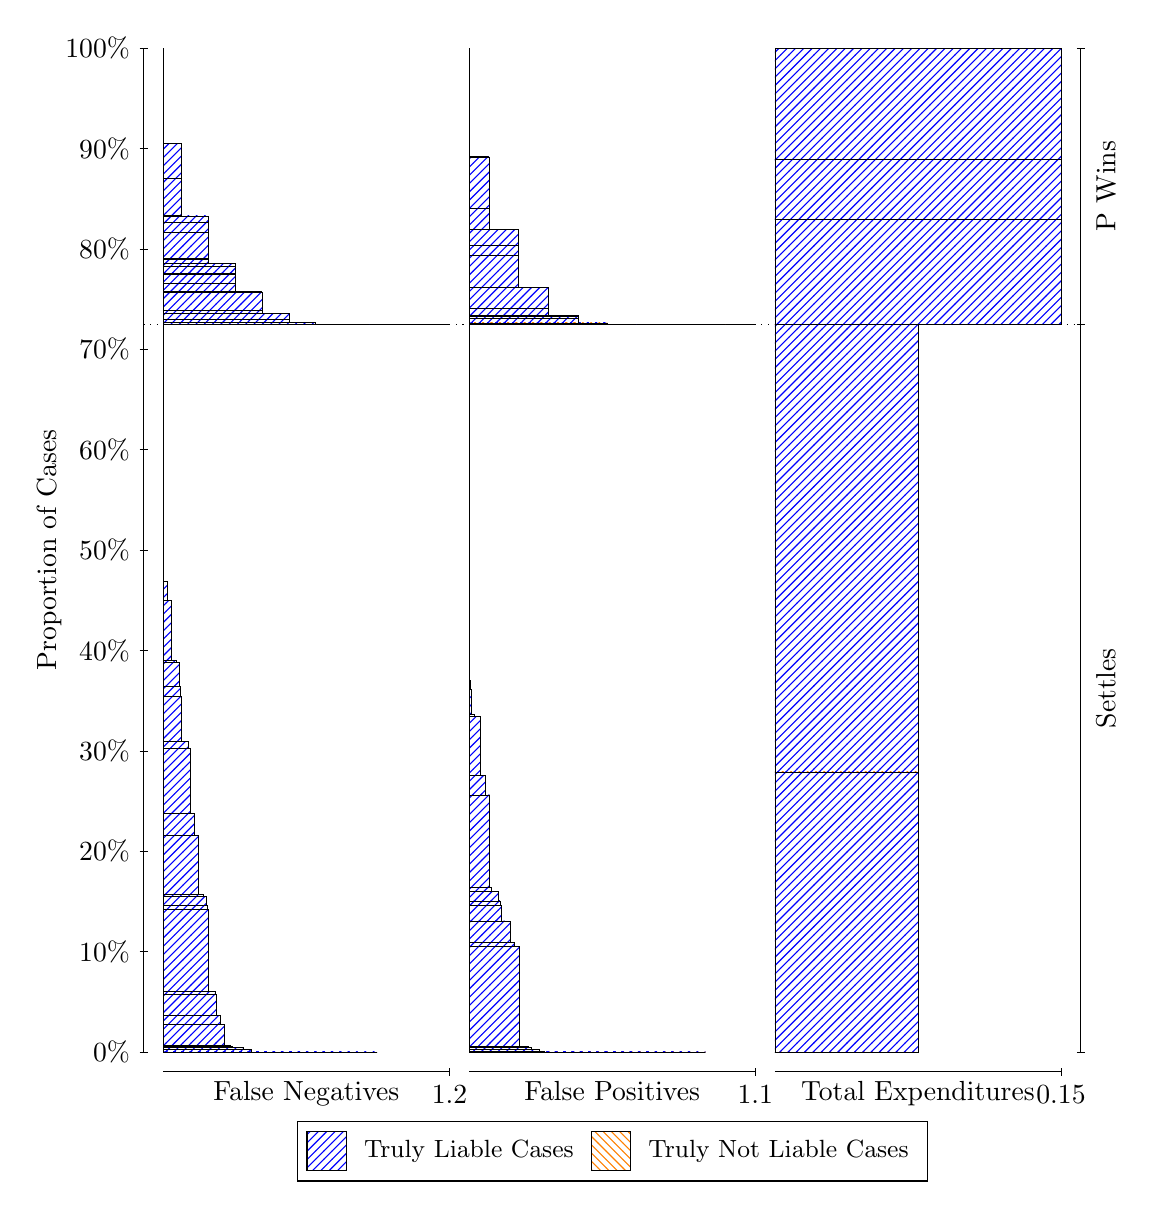
\begin{tikzpicture}
\draw[black, very thin] (1.5,1.75) -- (1.5,14.5);
\node[rotate=90, anchor=center] at (0.3, 8.125) {Proportion of Cases};
\draw[black, very thin] (1.45,1.75) -- (1.55,1.75);
\node[anchor=east] at (1.45, 1.75) {0\%};
\draw[black, very thin] (1.45,3.025) -- (1.55,3.025);
\node[anchor=east] at (1.45, 3.025) {10\%};
\draw[black, very thin] (1.45,4.3) -- (1.55,4.3);
\node[anchor=east] at (1.45, 4.3) {20\%};
\draw[black, very thin] (1.45,5.575) -- (1.55,5.575);
\node[anchor=east] at (1.45, 5.575) {30\%};
\draw[black, very thin] (1.45,6.85) -- (1.55,6.85);
\node[anchor=east] at (1.45, 6.85) {40\%};
\draw[black, very thin] (1.45,8.125) -- (1.55,8.125);
\node[anchor=east] at (1.45, 8.125) {50\%};
\draw[black, very thin] (1.45,9.4) -- (1.55,9.4);
\node[anchor=east] at (1.45, 9.4) {60\%};
\draw[black, very thin] (1.45,10.675) -- (1.55,10.675);
\node[anchor=east] at (1.45, 10.675) {70\%};
\draw[black, very thin] (1.45,11.95) -- (1.55,11.95);
\node[anchor=east] at (1.45, 11.95) {80\%};
\draw[black, very thin] (1.45,13.225) -- (1.55,13.225);
\node[anchor=east] at (1.45, 13.225) {90\%};
\draw[black, very thin] (1.45,14.5) -- (1.55,14.5);
\node[anchor=east] at (1.45, 14.5) {100\%};

\draw[black, very thin] (13.4,1.75) -- (13.4,14.5);
\draw[black, very thin] (13.35,1.75) -- (13.45,1.75);
\node[anchor=west] at (13.35, 1.75) {};
\draw[black, very thin] (13.35,10.99) -- (13.45,10.99);
\node[anchor=west] at (13.35, 10.99) {};
\draw[black, very thin] (13.35,14.5) -- (13.45,14.5);
\node[anchor=west] at (13.35, 14.5) {};

\draw[black, very thin, pattern color=blue, pattern=north east lines] (1.75,1.75) rectangle (4.4654,1.75);
\draw[black, very thin, pattern color=blue, pattern=north east lines] (1.75,1.75) rectangle (4.1255,1.75);
\draw[black, very thin, pattern color=blue, pattern=north east lines] (1.75,1.75) rectangle (4.0065,1.75);
\draw[black, very thin, pattern color=blue, pattern=north east lines] (1.75,1.75) rectangle (3.7855,1.75);
\draw[black, very thin, pattern color=blue, pattern=north east lines] (1.75,1.75) rectangle (3.6665,1.75);
\draw[black, very thin, pattern color=blue, pattern=north east lines] (1.75,1.75) rectangle (3.5475,1.75);
\draw[black, very thin, pattern color=blue, pattern=north east lines] (1.75,1.75) rectangle (3.4456,1.75);
\draw[black, very thin, pattern color=blue, pattern=north east lines] (1.75,1.75) rectangle (3.3946,1.75);
\draw[black, very thin, pattern color=blue, pattern=north east lines] (1.75,1.75) rectangle (3.3266,1.75);
\draw[black, very thin, pattern color=blue, pattern=north east lines] (1.75,1.75) rectangle (3.2076,1.7506);
\draw[black, very thin, pattern color=blue, pattern=north east lines] (1.75,1.7506) rectangle (3.1056,1.7511);
\draw[black, very thin, pattern color=blue, pattern=north east lines] (1.75,1.7511) rectangle (3.0886,1.7512);
\draw[black, very thin, pattern color=blue, pattern=north east lines] (1.75,1.7512) rectangle (3.0546,1.7512);
\draw[black, very thin, pattern color=blue, pattern=north east lines] (1.75,1.7512) rectangle (2.9866,1.7514);
\draw[black, very thin, pattern color=blue, pattern=north east lines] (1.75,1.7514) rectangle (2.9356,1.7518);
\draw[black, very thin, pattern color=blue, pattern=north east lines] (1.75,1.7518) rectangle (2.8676,1.7784);
\draw[black, very thin, pattern color=blue, pattern=north east lines] (1.75,1.7784) rectangle (2.7656,1.8046);
\draw[black, very thin, pattern color=blue, pattern=north east lines] (1.75,1.8046) rectangle (2.7486,1.8068);
\draw[black, very thin, pattern color=blue, pattern=north east lines] (1.75,1.8068) rectangle (2.7146,1.8068);
\draw[black, very thin, pattern color=blue, pattern=north east lines] (1.75,1.8068) rectangle (2.6466,1.8137);
\draw[black, very thin, pattern color=blue, pattern=north east lines] (1.75,1.8137) rectangle (2.6296,1.8245);
\draw[black, very thin, pattern color=blue, pattern=north east lines] (1.75,1.8245) rectangle (2.5957,1.8301);
\draw[black, very thin, pattern color=blue, pattern=north east lines] (1.75,1.8301) rectangle (2.5277,2.0997);
\draw[black, very thin, pattern color=blue, pattern=north east lines] (1.75,2.0997) rectangle (2.4767,2.2106);
\draw[black, very thin, pattern color=blue, pattern=north east lines] (1.75,2.2106) rectangle (2.4257,2.4824);
\draw[black, very thin, pattern color=blue, pattern=north east lines] (1.75,2.4824) rectangle (2.4087,2.5155);
\draw[black, very thin, pattern color=blue, pattern=north east lines] (1.75,2.5155) rectangle (2.3747,2.5155);
\draw[black, very thin, pattern color=blue, pattern=north east lines] (1.75,2.5155) rectangle (2.3237,3.556);
\draw[black, very thin, pattern color=blue, pattern=north east lines] (1.75,3.556) rectangle (2.3067,3.6144);
\draw[black, very thin, pattern color=blue, pattern=north east lines] (1.75,3.6144) rectangle (2.2897,3.7214);
\draw[black, very thin, pattern color=blue, pattern=north east lines] (1.75,3.7214) rectangle (2.2557,3.7475);
\draw[black, very thin, pattern color=blue, pattern=north east lines] (1.75,3.7475) rectangle (2.1877,4.5049);
\draw[black, very thin, pattern color=blue, pattern=north east lines] (1.75,4.5049) rectangle (2.1367,4.7814);
\draw[black, very thin, pattern color=blue, pattern=north east lines] (1.75,4.7814) rectangle (2.0857,5.6014);
\draw[black, very thin, pattern color=blue, pattern=north east lines] (1.75,5.6014) rectangle (2.0687,5.6965);
\draw[black, very thin, pattern color=blue, pattern=north east lines] (1.75,5.6965) rectangle (2.0347,5.6966);
\draw[black, very thin, pattern color=blue, pattern=north east lines] (1.75,5.6966) rectangle (1.9837,6.2679);
\draw[black, very thin, pattern color=blue, pattern=north east lines] (1.75,6.2679) rectangle (1.9667,6.3891);
\draw[black, very thin, pattern color=blue, pattern=north east lines] (1.75,6.3891) rectangle (1.9497,6.6979);
\draw[black, very thin, pattern color=blue, pattern=north east lines] (1.75,6.6979) rectangle (1.9157,6.7241);
\draw[black, very thin, pattern color=blue, pattern=north east lines] (1.75,6.7241) rectangle (1.8477,7.4816);
\draw[black, very thin, pattern color=blue, pattern=north east lines] (1.75,7.4816) rectangle (1.7967,7.7254);
\draw[black, very thin, pattern color=orange, pattern=north west lines] (1.75,7.7254) rectangle (1.75,7.7254);
\draw[black, very thin, pattern color=blue, pattern=north east lines] (1.75,7.7254) rectangle (1.75,10.99);
\draw[black, very thin, pattern color=blue, pattern=north east lines] (1.75,10.99) rectangle (5.3833,10.99);
\draw[black, very thin, pattern color=blue, pattern=north east lines] (1.75,10.99) rectangle (5.0434,10.99);
\draw[black, very thin, pattern color=blue, pattern=north east lines] (1.75,10.99) rectangle (4.7034,10.99);
\draw[black, very thin, pattern color=blue, pattern=north east lines] (1.75,10.99) rectangle (4.7034,10.99);
\draw[black, very thin, pattern color=blue, pattern=north east lines] (1.75,10.99) rectangle (4.3635,10.99);
\draw[black, very thin, pattern color=blue, pattern=north east lines] (1.75,10.99) rectangle (4.3635,10.99);
\draw[black, very thin, pattern color=blue, pattern=north east lines] (1.75,10.99) rectangle (4.3592,10.99);
\draw[black, very thin, pattern color=blue, pattern=north east lines] (1.75,10.99) rectangle (4.0235,10.992);
\draw[black, very thin, pattern color=blue, pattern=north east lines] (1.75,10.992) rectangle (4.0192,10.992);
\draw[black, very thin, pattern color=blue, pattern=north east lines] (1.75,10.992) rectangle (3.6835,11.014);
\draw[black, very thin, pattern color=blue, pattern=north east lines] (1.75,11.014) rectangle (3.6793,11.014);
\draw[black, very thin, pattern color=blue, pattern=north east lines] (1.75,11.014) rectangle (3.3436,11.054);
\draw[black, very thin, pattern color=blue, pattern=north east lines] (1.75,11.054) rectangle (3.3436,11.127);
\draw[black, very thin, pattern color=blue, pattern=north east lines] (1.75,11.127) rectangle (3.3393,11.127);
\draw[black, very thin, pattern color=blue, pattern=north east lines] (1.75,11.127) rectangle (3.3393,11.128);
\draw[black, very thin, pattern color=blue, pattern=north east lines] (1.75,11.128) rectangle (3.0036,11.166);
\draw[black, very thin, pattern color=blue, pattern=north east lines] (1.75,11.166) rectangle (3.0036,11.4);
\draw[black, very thin, pattern color=blue, pattern=north east lines] (1.75,11.4) rectangle (2.9994,11.403);
\draw[black, very thin, pattern color=blue, pattern=north east lines] (1.75,11.403) rectangle (2.9994,11.404);
\draw[black, very thin, pattern color=blue, pattern=north east lines] (1.75,11.404) rectangle (2.9994,11.408);
\draw[black, very thin, pattern color=blue, pattern=north east lines] (1.75,11.408) rectangle (2.6636,11.514);
\draw[black, very thin, pattern color=blue, pattern=north east lines] (1.75,11.514) rectangle (2.6636,11.631);
\draw[black, very thin, pattern color=blue, pattern=north east lines] (1.75,11.631) rectangle (2.6636,11.635);
\draw[black, very thin, pattern color=blue, pattern=north east lines] (1.75,11.635) rectangle (2.6594,11.645);
\draw[black, very thin, pattern color=blue, pattern=north east lines] (1.75,11.645) rectangle (2.6594,11.729);
\draw[black, very thin, pattern color=blue, pattern=north east lines] (1.75,11.729) rectangle (2.6594,11.761);
\draw[black, very thin, pattern color=blue, pattern=north east lines] (1.75,11.761) rectangle (2.3237,11.815);
\draw[black, very thin, pattern color=blue, pattern=north east lines] (1.75,11.815) rectangle (2.3194,11.833);
\draw[black, very thin, pattern color=blue, pattern=north east lines] (1.75,11.833) rectangle (2.3194,12.16);
\draw[black, very thin, pattern color=blue, pattern=north east lines] (1.75,12.16) rectangle (2.3194,12.29);
\draw[black, very thin, pattern color=blue, pattern=north east lines] (1.75,12.29) rectangle (2.3194,12.368);
\draw[black, very thin, pattern color=blue, pattern=north east lines] (1.75,12.368) rectangle (1.9837,12.368);
\draw[black, very thin, pattern color=blue, pattern=north east lines] (1.75,12.368) rectangle (1.9837,12.373);
\draw[black, very thin, pattern color=blue, pattern=north east lines] (1.75,12.373) rectangle (1.9837,12.373);
\draw[black, very thin, pattern color=blue, pattern=north east lines] (1.75,12.373) rectangle (1.9795,12.842);
\draw[black, very thin, pattern color=blue, pattern=north east lines] (1.75,12.842) rectangle (1.9795,13.289);
\draw[black, very thin, pattern color=orange, pattern=north west lines] (1.75,13.289) rectangle (1.75,13.289);
\draw[black, very thin, pattern color=blue, pattern=north east lines] (1.75,13.289) rectangle (1.75,14.5);
\draw[black, very thin, pattern color=orange, pattern=north west lines] (5.6333,1.75) rectangle (8.6329,1.75);
\draw[black, very thin, pattern color=blue, pattern=north east lines] (5.6333,1.75) rectangle (8.6329,1.75);
\draw[black, very thin, pattern color=orange, pattern=north west lines] (5.6333,1.75) rectangle (8.464,1.75);
\draw[black, very thin, pattern color=blue, pattern=north east lines] (5.6333,1.75) rectangle (8.464,1.75);
\draw[black, very thin, pattern color=orange, pattern=north west lines] (5.6333,1.75) rectangle (8.295,1.75);
\draw[black, very thin, pattern color=blue, pattern=north east lines] (5.6333,1.75) rectangle (8.295,1.75);
\draw[black, very thin, pattern color=blue, pattern=north east lines] (5.6333,1.75) rectangle (8.2574,1.75);
\draw[black, very thin, pattern color=blue, pattern=north east lines] (5.6333,1.75) rectangle (8.0884,1.75);
\draw[black, very thin, pattern color=orange, pattern=north west lines] (5.6333,1.75) rectangle (7.957,1.75);
\draw[black, very thin, pattern color=blue, pattern=north east lines] (5.6333,1.75) rectangle (7.957,1.75);
\draw[black, very thin, pattern color=blue, pattern=north east lines] (5.6333,1.75) rectangle (7.9194,1.75);
\draw[black, very thin, pattern color=blue, pattern=north east lines] (5.6333,1.75) rectangle (7.8819,1.75);
\draw[black, very thin, pattern color=orange, pattern=north west lines] (5.6333,1.75) rectangle (7.788,1.75);
\draw[black, very thin, pattern color=blue, pattern=north east lines] (5.6333,1.75) rectangle (7.788,1.75);
\draw[black, very thin, pattern color=blue, pattern=north east lines] (5.6333,1.75) rectangle (7.7129,1.75);
\draw[black, very thin, pattern color=blue, pattern=north east lines] (5.6333,1.75) rectangle (7.5814,1.75);
\draw[black, very thin, pattern color=blue, pattern=north east lines] (5.6333,1.75) rectangle (7.5439,1.75);
\draw[black, very thin, pattern color=blue, pattern=north east lines] (5.6333,1.75) rectangle (7.5063,1.75);
\draw[black, very thin, pattern color=orange, pattern=north west lines] (5.6333,1.75) rectangle (7.45,1.75);
\draw[black, very thin, pattern color=blue, pattern=north east lines] (5.6333,1.75) rectangle (7.45,1.75);
\draw[black, very thin, pattern color=blue, pattern=north east lines] (5.6333,1.75) rectangle (7.4124,1.75);
\draw[black, very thin, pattern color=blue, pattern=north east lines] (5.6333,1.75) rectangle (7.3373,1.75);
\draw[black, very thin, pattern color=orange, pattern=north west lines] (5.6333,1.75) rectangle (7.281,1.75);
\draw[black, very thin, pattern color=blue, pattern=north east lines] (5.6333,1.75) rectangle (7.281,1.75);
\draw[black, very thin, pattern color=blue, pattern=north east lines] (5.6333,1.75) rectangle (7.2059,1.75);
\draw[black, very thin, pattern color=blue, pattern=north east lines] (5.6333,1.75) rectangle (7.1683,1.75);
\draw[black, very thin, pattern color=blue, pattern=north east lines] (5.6333,1.75) rectangle (7.1308,1.75);
\draw[black, very thin, pattern color=blue, pattern=north east lines] (5.6333,1.75) rectangle (7.0745,1.75);
\draw[black, very thin, pattern color=blue, pattern=north east lines] (5.6333,1.75) rectangle (7.0369,1.75);
\draw[black, very thin, pattern color=blue, pattern=north east lines] (5.6333,1.75) rectangle (6.9618,1.75);
\draw[black, very thin, pattern color=blue, pattern=north east lines] (5.6333,1.75) rectangle (6.9055,1.7506);
\draw[black, very thin, pattern color=blue, pattern=north east lines] (5.6333,1.7506) rectangle (6.8304,1.7506);
\draw[black, very thin, pattern color=blue, pattern=north east lines] (5.6333,1.7506) rectangle (6.7928,1.7511);
\draw[black, very thin, pattern color=orange, pattern=north west lines] (5.6333,1.7511) rectangle (6.774,1.7511);
\draw[black, very thin, pattern color=blue, pattern=north east lines] (5.6333,1.7511) rectangle (6.774,1.7516);
\draw[black, very thin, pattern color=blue, pattern=north east lines] (5.6333,1.7516) rectangle (6.7553,1.7516);
\draw[black, very thin, pattern color=blue, pattern=north east lines] (5.6333,1.7516) rectangle (6.6989,1.7516);
\draw[black, very thin, pattern color=blue, pattern=north east lines] (5.6333,1.7516) rectangle (6.6614,1.7518);
\draw[black, very thin, pattern color=blue, pattern=north east lines] (5.6333,1.7518) rectangle (6.5863,1.7542);
\draw[black, very thin, pattern color=blue, pattern=north east lines] (5.6333,1.7542) rectangle (6.5299,1.7808);
\draw[black, very thin, pattern color=blue, pattern=north east lines] (5.6333,1.7808) rectangle (6.4548,1.7811);
\draw[black, very thin, pattern color=blue, pattern=north east lines] (5.6333,1.7811) rectangle (6.4173,1.8044);
\draw[black, very thin, pattern color=blue, pattern=north east lines] (5.6333,1.8044) rectangle (6.3985,1.8123);
\draw[black, very thin, pattern color=blue, pattern=north east lines] (5.6333,1.8123) rectangle (6.3797,1.8179);
\draw[black, very thin, pattern color=blue, pattern=north east lines] (5.6333,1.8179) rectangle (6.3234,1.818);
\draw[black, very thin, pattern color=blue, pattern=north east lines] (5.6333,1.818) rectangle (6.2858,1.8246);
\draw[black, very thin, pattern color=orange, pattern=north west lines] (5.6333,1.8246) rectangle (6.2671,1.8246);
\draw[black, very thin, pattern color=blue, pattern=north east lines] (5.6333,1.8246) rectangle (6.2671,3.0877);
\draw[black, very thin, pattern color=blue, pattern=north east lines] (5.6333,3.0877) rectangle (6.2107,3.1407);
\draw[black, very thin, pattern color=blue, pattern=north east lines] (5.6333,3.1407) rectangle (6.1544,3.4103);
\draw[black, very thin, pattern color=blue, pattern=north east lines] (5.6333,3.4103) rectangle (6.0793,3.4157);
\draw[black, very thin, pattern color=blue, pattern=north east lines] (5.6333,3.4157) rectangle (6.0417,3.6083);
\draw[black, very thin, pattern color=blue, pattern=north east lines] (5.6333,3.6083) rectangle (6.023,3.6674);
\draw[black, very thin, pattern color=blue, pattern=north east lines] (5.6333,3.6674) rectangle (6.0042,3.7854);
\draw[black, very thin, pattern color=blue, pattern=north east lines] (5.6333,3.7854) rectangle (5.9478,3.7855);
\draw[black, very thin, pattern color=blue, pattern=north east lines] (5.6333,3.7855) rectangle (5.9103,3.8384);
\draw[black, very thin, pattern color=blue, pattern=north east lines] (5.6333,3.8384) rectangle (5.8915,5.0142);
\draw[black, very thin, pattern color=blue, pattern=north east lines] (5.6333,5.0142) rectangle (5.8352,5.2581);
\draw[black, very thin, pattern color=blue, pattern=north east lines] (5.6333,5.2581) rectangle (5.7789,6.0155);
\draw[black, very thin, pattern color=blue, pattern=north east lines] (5.6333,6.0155) rectangle (5.7037,6.0417);
\draw[black, very thin, pattern color=blue, pattern=north east lines] (5.6333,6.0417) rectangle (5.6662,6.3505);
\draw[black, very thin, pattern color=blue, pattern=north east lines] (5.6333,6.3505) rectangle (5.6474,6.4718);
\draw[black, very thin, pattern color=blue, pattern=north east lines] (5.6333,6.4718) rectangle (5.6333,10.99);
\draw[black, very thin, pattern color=orange, pattern=north west lines] (5.6333,10.99) rectangle (9.2667,10.99);
\draw[black, very thin, pattern color=blue, pattern=north east lines] (5.6333,10.99) rectangle (9.2667,10.99);
\draw[black, very thin, pattern color=orange, pattern=north west lines] (5.6333,10.99) rectangle (8.8911,10.99);
\draw[black, very thin, pattern color=blue, pattern=north east lines] (5.6333,10.99) rectangle (8.8911,10.99);
\draw[black, very thin, pattern color=orange, pattern=north west lines] (5.6333,10.99) rectangle (8.5156,10.99);
\draw[black, very thin, pattern color=blue, pattern=north east lines] (5.6333,10.99) rectangle (8.5156,10.99);
\draw[black, very thin, pattern color=blue, pattern=north east lines] (5.6333,10.99) rectangle (8.5156,10.99);
\draw[black, very thin, pattern color=blue, pattern=north east lines] (5.6333,10.99) rectangle (8.1401,10.99);
\draw[black, very thin, pattern color=orange, pattern=north west lines] (5.6333,10.99) rectangle (8.1401,10.99);
\draw[black, very thin, pattern color=blue, pattern=north east lines] (5.6333,10.99) rectangle (8.1401,10.99);
\draw[black, very thin, pattern color=orange, pattern=north west lines] (5.6333,10.99) rectangle (7.7645,10.99);
\draw[black, very thin, pattern color=blue, pattern=north east lines] (5.6333,10.99) rectangle (7.7645,10.992);
\draw[black, very thin, pattern color=orange, pattern=north west lines] (5.6333,10.992) rectangle (7.7598,10.992);
\draw[black, very thin, pattern color=blue, pattern=north east lines] (5.6333,10.992) rectangle (7.7598,10.992);
\draw[black, very thin, pattern color=orange, pattern=north west lines] (5.6333,10.992) rectangle (7.389,10.992);
\draw[black, very thin, pattern color=blue, pattern=north east lines] (5.6333,10.992) rectangle (7.389,11.008);
\draw[black, very thin, pattern color=orange, pattern=north west lines] (5.6333,11.008) rectangle (7.3843,11.008);
\draw[black, very thin, pattern color=blue, pattern=north east lines] (5.6333,11.008) rectangle (7.3843,11.008);
\draw[black, very thin, pattern color=blue, pattern=north east lines] (5.6333,11.008) rectangle (7.3843,11.008);
\draw[black, very thin, pattern color=orange, pattern=north west lines] (5.6333,11.008) rectangle (7.0134,11.008);
\draw[black, very thin, pattern color=blue, pattern=north east lines] (5.6333,11.008) rectangle (7.0134,11.064);
\draw[black, very thin, pattern color=blue, pattern=north east lines] (5.6333,11.064) rectangle (7.0134,11.092);
\draw[black, very thin, pattern color=blue, pattern=north east lines] (5.6333,11.092) rectangle (7.0134,11.108);
\draw[black, very thin, pattern color=blue, pattern=north east lines] (5.6333,11.108) rectangle (7.0087,11.108);
\draw[black, very thin, pattern color=orange, pattern=north west lines] (5.6333,11.108) rectangle (7.0087,11.108);
\draw[black, very thin, pattern color=blue, pattern=north east lines] (5.6333,11.108) rectangle (7.0087,11.108);
\draw[black, very thin, pattern color=orange, pattern=north west lines] (5.6333,11.108) rectangle (6.6379,11.108);
\draw[black, very thin, pattern color=blue, pattern=north east lines] (5.6333,11.108) rectangle (6.6379,11.191);
\draw[black, very thin, pattern color=blue, pattern=north east lines] (5.6333,11.191) rectangle (6.6379,11.459);
\draw[black, very thin, pattern color=blue, pattern=north east lines] (5.6333,11.459) rectangle (6.6332,11.459);
\draw[black, very thin, pattern color=orange, pattern=north west lines] (5.6333,11.459) rectangle (6.6332,11.459);
\draw[black, very thin, pattern color=blue, pattern=north east lines] (5.6333,11.459) rectangle (6.6332,11.459);
\draw[black, very thin, pattern color=blue, pattern=north east lines] (5.6333,11.459) rectangle (6.2624,11.866);
\draw[black, very thin, pattern color=blue, pattern=north east lines] (5.6333,11.866) rectangle (6.2624,11.996);
\draw[black, very thin, pattern color=blue, pattern=north east lines] (5.6333,11.996) rectangle (6.2624,12.201);
\draw[black, very thin, pattern color=blue, pattern=north east lines] (5.6333,12.201) rectangle (6.2577,12.201);
\draw[black, very thin, pattern color=orange, pattern=north west lines] (5.6333,12.201) rectangle (6.2577,12.201);
\draw[black, very thin, pattern color=blue, pattern=north east lines] (5.6333,12.201) rectangle (6.2577,12.201);
\draw[black, very thin, pattern color=blue, pattern=north east lines] (5.6333,12.201) rectangle (5.8868,12.463);
\draw[black, very thin, pattern color=blue, pattern=north east lines] (5.6333,12.463) rectangle (5.8868,13.117);
\draw[black, very thin, pattern color=blue, pattern=north east lines] (5.6333,13.117) rectangle (5.8821,13.117);
\draw[black, very thin, pattern color=blue, pattern=north east lines] (5.6333,13.117) rectangle (5.8821,13.118);
\draw[black, very thin, pattern color=orange, pattern=north west lines] (5.6333,13.118) rectangle (5.8821,13.118);
\draw[black, very thin, pattern color=blue, pattern=north east lines] (5.6333,13.118) rectangle (5.8821,13.121);
\draw[black, very thin, pattern color=blue, pattern=north east lines] (5.6333,13.121) rectangle (5.8821,13.121);
\draw[black, very thin, pattern color=orange, pattern=north west lines] (5.6333,13.121) rectangle (5.6333,13.121);
\draw[black, very thin, pattern color=blue, pattern=north east lines] (5.6333,13.121) rectangle (5.6333,14.5);
\draw[black, very thin, pattern color=orange, pattern=north west lines] (9.5167,1.75) rectangle (11.333,1.75);
\draw[black, very thin, pattern color=blue, pattern=north east lines] (9.5167,1.75) rectangle (11.333,5.3077);
\draw[black, very thin, pattern color=orange, pattern=north west lines] (9.5167,5.3077) rectangle (11.333,5.3077);
\draw[black, very thin, pattern color=blue, pattern=north east lines] (9.5167,5.3077) rectangle (11.333,10.99);
\draw[black, very thin, pattern color=orange, pattern=north west lines] (9.5167,10.99) rectangle (13.15,10.99);
\draw[black, very thin, pattern color=blue, pattern=north east lines] (9.5167,10.99) rectangle (13.15,12.328);
\draw[black, very thin, pattern color=orange, pattern=north west lines] (9.5167,12.328) rectangle (13.15,12.328);
\draw[black, very thin, pattern color=blue, pattern=north east lines] (9.5167,12.328) rectangle (13.15,13.082);
\draw[black, very thin, pattern color=orange, pattern=north west lines] (9.5167,13.082) rectangle (13.15,13.082);
\draw[black, very thin, pattern color=blue, pattern=north east lines] (9.5167,13.082) rectangle (13.15,14.5);
\draw[black, dotted] (1.5,10.99) -- (13.4,10.99);
\draw[black, very thin] (1.75,1.5) -- (5.3833,1.5);
\node[anchor=north] at (3.5667, 1.5) {False Negatives};
\draw[black, very thin] (5.3833,1.45) -- (5.3833,1.55);
\node[anchor=north] at (5.3833, 1.45) {1.2};

\draw[black, very thin] (5.6333,1.5) -- (9.2667,1.5);
\node[anchor=north] at (7.45, 1.5) {False Positives};
\draw[black, very thin] (9.2667,1.45) -- (9.2667,1.55);
\node[anchor=north] at (9.2667, 1.45) {1.1};

\draw[black, very thin] (9.5167,1.5) -- (13.15,1.5);
\node[anchor=north] at (11.333, 1.5) {Total Expenditures};
\draw[black, very thin] (13.15,1.45) -- (13.15,1.55);
\node[anchor=north] at (13.15, 1.45) {0.15};

\node[black, centered, rotate=90] at (13.72, 6.3698) {Settles};
\node[black, centered, rotate=90] at (13.72, 12.745) {P Wins};

\draw (7.449999999999999,1.5) node[draw=none] (baseCoordinate) {};
\begin{scope}[align=center]
        \matrix[scale=0.5, draw=black, below=0.5cm of baseCoordinate, nodes={draw}, column sep=0.1cm]{
            \node[rectangle, draw, minimum width=0.5cm, minimum height=0.5cm, pattern=north east lines, pattern color=blue] {}; &
            \node[draw=none, font=\small] (B) {Truly Liable Cases}; &
            \node[rectangle, draw, minimum width=0.5cm, minimum height=0.5cm, pattern=north west lines, pattern color=orange] {}; &
            \node[draw=none, font=\small] (B) {Truly Not Liable Cases}; \\
            };
\end{scope}

\end{tikzpicture}
\end{document}